\documentclass{article}
\usepackage{tikz}
\usetikzlibrary{calc,scopes}
\usepackage{hyperref}
\usepackage[margin=1in]{geometry}

\begin{document}

% MRNG-Based Graph Construction and Nearest Neighbor Search

\section*{Limitations of MRNG for Nearest Neighbor Search: A Lune-Based Example}

\begin{figure}[ht]
    \centering
    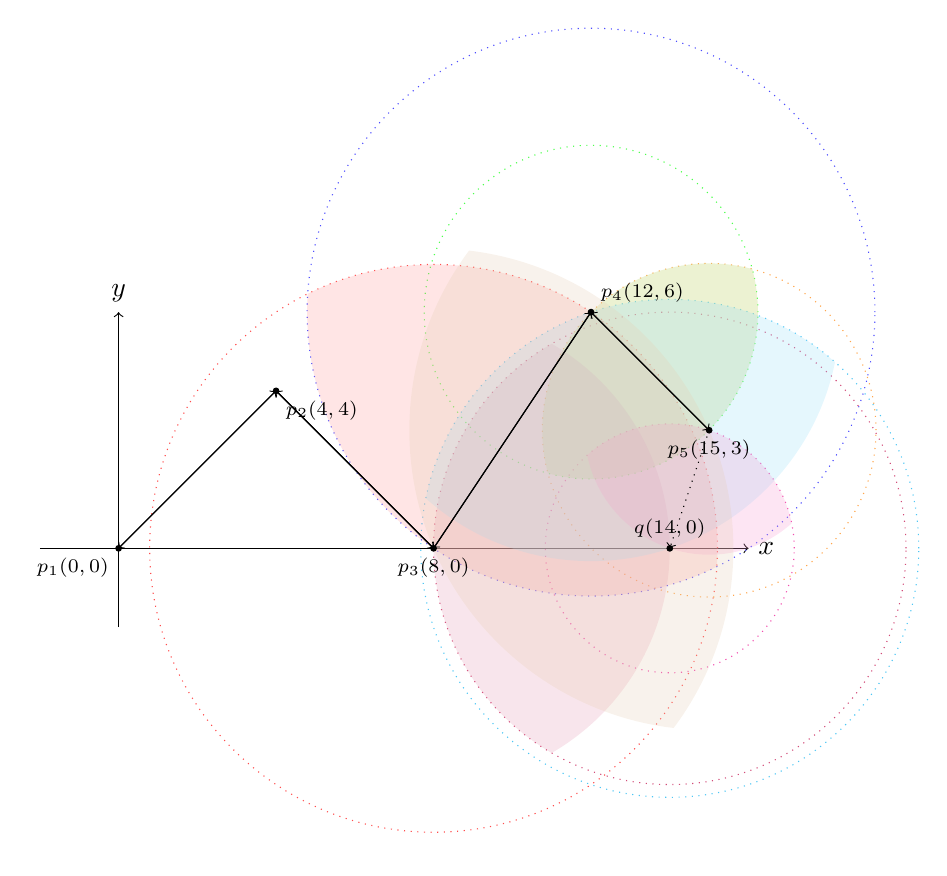
\begin{tikzpicture}[scale=0.5]
        % Define coordinates
        \coordinate (p1) at (0,0);
        \coordinate (p2) at (4,4);
        \coordinate (p3) at (8,0);
        % Update p4 coordinate and label
        \coordinate (p4) at (12,6);
        % Update p5 coordinate and label
        \coordinate (p5) at (15,3);
        \coordinate (q) at (14,0);

        % Draw axes
        \draw[->] (-2,0) -- (16,0) node[right] {$x$};
        \draw[->] (0,-2) -- (0,6) node[above] {$y$};

        % Draw all circles as before, but with slightly darker, soft boundaries
        \draw[red!70, dotted, thin] let \p1=(p3), \p2=(p4), \n1={veclen(\x2-\x1,\y2-\y1)} in (p3) circle (\n1);
        \draw[blue!70, dotted, thin] let \p1=(p4), \p2=(p3), \n1={veclen(\x2-\x1,\y2-\y1)} in (p4) circle (\n1);
        \draw[green!70, dotted, thin] let \p1=(p4), \p2=(p5), \n1={veclen(\x2-\x1,\y2-\y1)} in (p4) circle (\n1);
        \draw[orange!70, dotted, thin] let \p1=(p5), \p2=(p4), \n1={veclen(\x2-\x1,\y2-\y1)} in (p5) circle (\n1);
        % Draw the new circles for q
        \draw[purple!70, dotted, thin] let \p1=(q), \p2=(p3), \n1={veclen(\x2-\x1,\y2-\y1)} in (q) circle (\n1);
        \draw[cyan!70, dotted, thin] let \p1=(q), \p2=(p4), \n1={veclen(\x2-\x1,\y2-\y1)} in (q) circle (\n1);
        \draw[magenta!70, dotted, thin] let \p1=(q), \p2=(p5), \n1={veclen(\x2-\x1,\y2-\y1)} in (q) circle (\n1);

        % Update all lune fills to be a bit darker
        % Lune between circle centered at p3 and p4 (excluding overlap with p5)
        \begin{scope}
            \clip let \p1=(p3), \p2=(p4), \n1={veclen(\x2-\x1,\y2-\y1)} in (p3) circle (\n1);
            \path[fill=red!40, fill opacity=0.25, draw=none] let \p1=(p4), \p2=(p3), \n1={veclen(\x2-\x1,\y2-\y1)} in (p4) circle (\n1);
        \end{scope}
        % Lune between circle centered at p4 and p5 (excluding overlap with p3)
        \begin{scope}
            \clip let \p1=(p4), \p2=(p5), \n1={veclen(\x2-\x1,\y2-\y1)} in (p4) circle (\n1);
            \path[fill=green!40, fill opacity=0.25, draw=none] let \p1=(p5), \p2=(p4), \n1={veclen(\x2-\x1,\y2-\y1)} in (p5) circle (\n1);
        \end{scope}
        % Lune between circle centered at p5 and p4 (excluding overlap with p3)
        \begin{scope}
            \clip let \p1=(p5), \p2=(p4), \n1={veclen(\x2-\x1,\y2-\y1)} in (p5) circle (\n1);
            \path[fill=orange!40, fill opacity=0.25, draw=none] let \p1=(p4), \p2=(p5), \n1={veclen(\x2-\x1,\y2-\y1)} in (p4) circle (\n1);
        \end{scope}
        % Lune between circle centered at q and p3
        \begin{scope}
            \clip let \p1=(q), \p2=(p3), \n1={veclen(\x2-\x1,\y2-\y1)} in (q) circle (\n1);
            \path[fill=purple!40, fill opacity=0.25, draw=none] let \p1=(p3), \p2=(q), \n1={veclen(\x2-\x1,\y2-\y1)} in (p3) circle (\n1);
        \end{scope}
        % Lune between circle centered at q and p4
        \begin{scope}
            \clip let \p1=(q), \p2=(p4), \n1={veclen(\x2-\x1,\y2-\y1)} in (q) circle (\n1);
            \path[fill=cyan!40, fill opacity=0.25, draw=none] let \p1=(p4), \p2=(q), \n1={veclen(\x2-\x1,\y2-\y1)} in (p4) circle (\n1);
        \end{scope}
        % Lune between circle centered at q and p5
        \begin{scope}
            \clip let \p1=(q), \p2=(p5), \n1={veclen(\x2-\x1,\y2-\y1)} in (q) circle (\n1);
            \path[fill=magenta!40, fill opacity=0.25, draw=none] let \p1=(p5), \p2=(q), \n1={veclen(\x2-\x1,\y2-\y1)} in (p5) circle (\n1);
        \end{scope}
        % Lune between circle centered at p3 and p5
        \begin{scope}
            \clip let \p1=(p3), \p2=(p5), \n1={veclen(\x2-\x1,\y2-\y1)} in (p3) circle (\n1);
            \path[fill=brown!40, fill opacity=0.25, draw=none] let \p1=(p5), \p2=(p3), \n1={veclen(\x2-\x1,\y2-\y1)} in (p5) circle (\n1);
        \end{scope}

        % Draw directed edges on top of circles/shadings, but below points
        \draw[->, thin] (p1) -- (p2);
        \draw[->, thin] (p2) -- (p1);
        \draw[->, thin] (p2) -- (p3);
        \draw[->, thin] (p3) -- (p2);
        \draw[->, thin] (p3) -- (p4);
        \draw[->, thin] (p4) -- (p3);
        \draw[->, thin] (p4) -- (p5);
        \draw[->, thin] (p5) -- (p4);
        \draw[->, dotted, thin] (p5) -- (q);

        % Draw points on top of everything else, with smaller coordinate labels
        \filldraw (p1) circle (2pt) node[below left] {\scriptsize $p_1(0,0)$};
        \filldraw (p2) circle (2pt) node[below right] {\scriptsize $p_2(4,4)$};
        \filldraw (p3) circle (2pt) node[below] {\scriptsize $p_3(8,0)$};
        \filldraw (p4) circle (2pt) node[above right] {\scriptsize $p_4(12,6)$};
        \filldraw (p5) circle (2pt) node[below] {\scriptsize $p_5(15,3)$};
        \filldraw (q) circle (2pt) node[above] {\scriptsize $q(14,0)$};
    \end{tikzpicture}
    \caption{MRNG-based graph construction and nearest neighbor search.}
    \label{fig:mrng-diagram}
\end{figure}

\noindent This document illustrates the construction of a graph using the \textbf{Monotonic Relative Neighborhood Graph (MRNG)} for a set of points $p_1, p_2, p_3, p_4, p_5$. It also demonstrates how the graph is used to search for the nearest neighbor to a query point $q$, which is \textbf{not} part of the original graph. See Figure~\autoref{fig:mrng-diagram}.

\subsection*{MRNG Construction}
\begin{itemize}
    \item \textbf{Vertices:} The points $p_1, p_2, p_3, p_4, p_5$ are the vertices of the graph.
    \item \textbf{Directed Edges:} For each point, all other points are sorted by distance. A directed edge from $u$ to $v$ is added if, within the lune (the intersection of the circles centered at $u$ and $v$ passing through each other), there is no other point $w$ such that an edge from $u$ to $w$ already exists and $w$ is closer to $u$ than $v$.
    \item \textbf{Lunes:} The shaded regions in the diagram represent the lunes for each pair of points. \\ 
    \textit{The lune here helps understand which points are closer: if a third point $w$ exists inside the lune of vertices $u$ and $v$, then $w$ is closer to both $u$ and $v$ than they are to each other.} This property is used to decide whether a direct edge should be formed between $u$ and $v$.
\end{itemize}

\newpage
\subsection*{Query Point and Search}
\begin{itemize}
    \item \textbf{Query Point $q$:} The point $q$ is not part of the original graph.
    \item \textbf{Search Process:} To find the nearest neighbor to $q$, the search starts from a given vertex (e.g., $p_1$) and, at each step, moves to the neighbor that is greedily closer to $q$. The process stops when no neighbor is closer to $q$ than the current point.
    \item \textbf{MRNG Navigability:} MRNG guarantees that every point in the graph is reachable from every other point (all-point navigability). However, this guarantee does \textbf{not} extend to query points that are not part of the graph.
\end{itemize}

\subsection*{Observation}
\begin{itemize}
    \item In the illustrated example, if the search for the nearest neighbor to $q$ starts at $p_1$, the search path is:
    \begin{itemize}
        \item $p_1 \rightarrow p_2 \rightarrow p_3$
        \item The search stops at $p_3$ because none of its neighbors are closer to $q$.
        \item However, the true nearest neighbor to $q$ is $p_5$, not $p_3$.
    \end{itemize}
    \item \textbf{Conclusion:} MRNG does \textbf{not} guarantee that the nearest neighbor search will succeed for query points not in the graph, even though it guarantees navigability for all points within the graph.
\end{itemize}

\subsection*{Summary}
\begin{itemize}
    \item \textbf{MRNG} is useful for constructing navigable graphs for a set of points.
    \item \textbf{Nearest neighbor search} using MRNG may fail for external query points, as shown in the diagram.
    \item \textbf{Practical implication:} For applications like approximate nearest neighbor search, additional strategies may be needed to ensure correct results for queries outside the original dataset.
\end{itemize}

\end{document}
